% Match Me If You Can: Privacy-Preserving Registration via STARK-STIR
% Paper outline / draft scaffold.

\documentclass[11pt,a4paper]{article}

\usepackage[utf8]{inputenc}
\usepackage[T1]{fontenc}
\usepackage[margin=1in]{geometry}
\usepackage{microtype}
\usepackage{booktabs}
\usepackage{multirow}
\usepackage{siunitx}
\sisetup{group-separator={,}, group-minimum-digits=4}
\usepackage{amsmath, amssymb, amsthm}
\usepackage{xcolor}
\usepackage{hyperref}
\usepackage{tikz}
\usepackage{pgfplots}
\pgfplotsset{compat=1.18}
\usepackage{algorithm, algpseudocode}

\hypersetup{
  colorlinks   = true,
  linkcolor    = blue!50!black,
  citecolor    = blue!50!black,
  urlcolor     = blue!50!black,
}

\newtheorem{theorem}{Theorem}
\newtheorem{definition}{Definition}
\newtheorem{property}{Property}

\title{
  Match Me If You Can: \\
  Privacy-Preserving Registration via STARK-STIR Proofs over PII
}
\author{Stephen A. Holmes \\
  University of Surrey \\
  \texttt{s.a.holmes@surrey.ac.uk}}
\date{2026}

\begin{document}

\maketitle

\begin{abstract}
% A precise four-axis claim — keep tight after the empirical numbers come in.
A typical website registration flow stores user attributes — date of
birth, country, postcode, email, income — verbatim in a database.  When
that database is breached, the leaked records are linkable against
publicly-available auxiliary data (electoral rolls, breach corpora,
social-media exports), and the operator faces UK / EU GDPR fines
under Art.~83.  We replace the verbatim attribute columns with
\textbf{STARK-STIR proofs of attribute predicates} — range proofs and
set-membership proofs constructed using the post-quantum,
no-trusted-setup STARK-STIR protocol of \cite{stark-stir}.  The server
answers every business-relevant query
(``authorised?''~``in~the~EU?''~``over~18?'') by re-verifying the
stored proof; the underlying value is never present in the database to
be leaked.  We empirically quantify four cost / benefit axes:
storage (bytes per user), compute (prove and verify latency), breach
unlinkability (re-identification rate against an auxiliary database),
and regulatory cost (expected GDPR fine differential, weighted by
per-year breach probability).  All numbers are reproducible from the
open-source reference implementation~\cite{mmiyc-impl}.
\end{abstract}

\section{Introduction}
\label{sec:intro}

Industrial-scale data breaches are routine.  The UK Information
Commissioner's Office issues administrative penalties for around
150 reportable incidents per year~\cite{ico-fines}; the
2024 Ponemon / IBM \emph{Cost of a Data Breach Report} puts the
global mean cost at \$165 (\$\approx \pounds 130$) per affected
record.  Under UK and EU GDPR, the structural protection that
operators are expected to deploy is
\emph{pseudonymisation}~(Art.~4(5))~\cite{gdpr,uk-gdpr} — but
in practice this almost always collapses to ``encrypt the column at
rest'', which leaks the moment the encryption key is compromised
or the database is read by an authorised but unintended principal.
The leaked records are typically rich enough to be
\emph{linked} against publicly-available auxiliary data
(electoral rolls, breach corpora, social-media exports), at which
point the well-known re\nobreakdash-identification result of
\cite{sweeney2000simple} applies: 87~\% of the population is
uniquely identifiable by ZIP + DOB + sex alone.

This paper makes the case that for many attributes captured at
registration, the operator does not need the value — they need a
\emph{predicate over the value}.  ``Are you over 18?''~is a one-bit
question; storing the full date of birth to answer it is
over\nobreakdash-collection.  We show that replacing verbatim PII with
STARK\nobreakdash-STIR proofs of the relevant predicates
\cite{stark-stir,stir,starks} reduces breach\nobreakdash-time exposure
to informational zero (in the cryptographic sense) and produces a
quantifiable reduction in expected regulatory cost.

\paragraph{Contributions.}

\begin{enumerate}
  \item A \textbf{registration architecture} that replaces verbatim
        PII storage with on\nobreakdash-disk STARK\nobreakdash-STIR
        proofs of attribute predicates (\S\ref{sec:design}).
  \item A set of \textbf{AIRs} for common registration predicates —
        age range, country set membership, postcode prefix membership,
        email\nobreakdash-domain membership, income bracket — built on
        the post\nobreakdash-quantum, no\nobreakdash-trusted\nobreakdash-setup
        STARK\nobreakdash-STIR construction of
        \cite{stark-stir} (\S\ref{sec:airs}).
  \item An \textbf{empirical four\nobreakdash-axis evaluation}:
        storage, compute, breach unlinkability, and regulatory cost
        (\S\ref{sec:eval}).  Evaluated on a synthetic
        $10{,}000$\textendash$100{,}000$\nobreakdash-user UK
        population.  Headline numbers: $220\!\times$ storage
        overhead, $29.3\,\%$ vs $0\,\%$ re\nobreakdash-identification,
        and $\sim\!\pounds 19{,}000$\nobreakdash-per\nobreakdash-year
        expected\nobreakdash-fine reduction per $10{,}000$ users at
        baseline parameters.
  \item A \textbf{breach simulation} that quantifies
        re\nobreakdash-identification rate under both scenarios against
        a public auxiliary database, and a
        \textbf{regulatory\nobreakdash-cost analysis} that translates
        that rate into an expected GDPR Art.~83 fine differential
        with sensitivity sweeps over breach probability and per\nobreakdash-record
        cost (\S\ref{sec:eval-regulatory}).
  \item An \textbf{open\nobreakdash-source reference implementation} —
        Rust workspace, $\sim\!1{,}500$ lines of pure Rust plus
        $\sim\!250$ lines of LaTeX, all benchmarks and analyses
        reproducible from the
        repository~\cite{mmiyc-impl}.
\end{enumerate}

% ──────────────────────────────────────────────────────────────────
\begin{figure}[h]
  \centering
  \begin{tikzpicture}[
    node distance = 0.6cm and 1cm,
    box/.style    = {rectangle, draw=black!60, thick, rounded corners=2pt,
                     minimum width=3.4cm, minimum height=0.7cm,
                     align=center, font=\small},
    db/.style     = {cylinder, shape border rotate=90, draw=black!60, thick,
                     aspect=0.3, minimum height=1.4cm, minimum width=2.6cm,
                     align=center, font=\small},
    arrow/.style  = {-stealth, thick}
  ]
    % Top row — user / browser
    \node[box,fill=blue!8]   (user)  {User browser \\ (registration form)};
    % Server
    \node[box,fill=orange!8, below=of user] (server) {Service backend};
    % Two storage scenarios side-by-side
    \node[db, fill=red!8,  below left=of server, xshift=-1cm] (pii)    {{\bf PII} \\ {\footnotesize raw values \\ encrypted at rest}};
    \node[db, fill=green!8,below right=of server, xshift=1cm] (proofs) {{\bf Proofs} \\ {\footnotesize STARK-STIR proof \\ bytes only}};
    % Adversary
    \node[box, fill=black!8, right=of proofs, xshift=0.4cm] (adv) {Breach adversary \\ + auxiliary DB};
    % Arrows
    \draw[arrow] (user)   -- (server)  node[midway,right]{\footnotesize attributes};
    \draw[arrow] (server) -- (pii)     node[midway,sloped,below]{\footnotesize \emph{baseline}};
    \draw[arrow] (server) -- (proofs)  node[midway,sloped,above]{\footnotesize \emph{proposed}};
    \draw[arrow, dashed, red!70] (pii.east)    -- (adv.west) node[midway,above]{\footnotesize linkage};
    \draw[arrow, dashed, green!50!black, ultra thin] (proofs.east) -- (adv.west) node[midway,below]{\footnotesize \emph{no handles}};
  \end{tikzpicture}
  \caption{The two storage scenarios share the same registration
  UX but differ in what the database stores.  Under
  PII\nobreakdash-storage, a breach hands the adversary attribute
  tuples that link directly against any auxiliary database with
  the same fields.  Under proof\nobreakdash-storage, the adversary
  obtains only STARK\nobreakdash-STIR proof bytes, which carry no
  exploitable attribute information.}
  \label{fig:two-scenarios}
\end{figure}

\section{Background}
\label{sec:background}

\paragraph{STARKs and STIR.}  A STARK is a
Scalable Transparent ARgument of Knowledge: a
non\nobreakdash-interactive proof system with poly\nobreakdash-logarithmic
verifier complexity, no trusted setup, and post\nobreakdash-quantum
soundness~\cite{starks}.  The proof attests that a witness
$w$ satisfies the constraints of an Algebraic Intermediate
Representation (AIR), where the AIR is encoded as a set of
low\nobreakdash-degree polynomial constraints over a finite field.
Standard pipelines reduce constraint satisfaction to a low\nobreakdash-degree
test on a Reed--Solomon code; STIR~\cite{stir} is a recent
construction of that low\nobreakdash-degree test with substantially
fewer queries than FRI for equivalent soundness.  We use the
STARK\nobreakdash-STIR composite construction
of \cite{stark-stir} both for the AIR machinery
and the final low\nobreakdash-degree test.

\paragraph{AIRs.}  An AIR is a tuple
$(W,\ T,\ C_\mathrm{transition},\ C_\mathrm{boundary})$ where
$W$ is the trace width (number of columns), $T$ is the trace
length (number of rows), $C_\mathrm{transition}$ is a set of
polynomial constraints relating consecutive rows, and
$C_\mathrm{boundary}$ pins specific cells.  Each AIR in
\S\ref{sec:airs} is presented in this form.

\paragraph{UK / EU GDPR.}  The relevant articles for the
regulatory analysis: Art.~4(5) defines pseudonymisation;
Art.~32 enumerates appropriate security measures
(``encryption and pseudonymisation'' is the canonical pair);
Art.~33--34 governs breach notification (relaxed when the data
is unintelligible); Art.~83 sets fines up to the greater of
\euro20\,M or $4\,\%$ of global annual
turnover~\cite{gdpr,uk-gdpr,ico-fines}.  Our cost model in
\S\ref{sec:eval-regulatory} treats Art.~83 as the binding
fine schedule and uses ICO\nobreakdash-published precedent for
the per\nobreakdash-record cost.

\section{Threat Model and Design Goals}
\label{sec:threat}

\paragraph{Setting.}  A standard web application (registration,
login, account management) handling personally\nobreakdash-identifiable
information.  The operator is a typical SaaS business or
public\nobreakdash-facing service subject to UK / EU GDPR.  The
user population is the general public.

\paragraph{Adversary.}  A passive observer with full read access
to the at\nobreakdash-rest database, plus the ability to consult
publicly\nobreakdash-available auxiliary databases (electoral\nobreakdash-roll
snapshots, breach corpora, social\nobreakdash-media exports, voter
registration data, commercial data brokers).  This is the
classical \emph{honest\nobreakdash-but\nobreakdash-curious database breach}:
the adversary does not actively interfere with the service, but at
some moment they obtain a complete read snapshot of the back\nobreakdash-end
store.  They then attempt to \emph{link} records in the breach to
identities in the auxiliary databases, completing the picture and
enabling identity theft, targeted phishing, or regulatory weaponisation.
The adversary is bounded by classical computation for the
breach\nobreakdash-window analysis but is additionally assumed
post\nobreakdash-quantum\nobreakdash-capable for forward\nobreakdash-secrecy
claims about the proof storage — one of STARK\nobreakdash-STIR's selling
points.

\paragraph{Out of scope.}  Active service compromise (an attacker
with code\nobreakdash-execution on the service can intercept PII
before the proof is generated; mitigations via TEE or
client\nobreakdash-side WASM prover are noted as future work in
\S\ref{sec:discussion}); side channels in the prover; targeted
legal compulsion; and verifier\nobreakdash-side query\nobreakdash-log
leakage.

\paragraph{Security claim (informal).}  For each PII attribute
stored under the proof scenario, an adversary holding the breach
data alone (no auxiliary information) cannot recover the
attribute's value with non\nobreakdash-negligible probability beyond
the prior distribution of that attribute over the user population.
Specifically: a range\nobreakdash-proof of ``age $\geq 18$'' reveals no
information beyond
$\Pr\bigl[\mathrm{age} \geq 18 \mid \mathrm{user\_population}\bigr]$
plus the verifier's published policy binding; a
set\nobreakdash-membership proof of ``country $\in$ EU'' reveals no
information beyond
$\Pr\bigl[\mathrm{country} \in \mathrm{EU} \mid \mathrm{user\_population}\bigr]$.
The classical STARK soundness and zero\nobreakdash-knowledge properties
of STARK\nobreakdash-STIR \cite{stark-stir} underwrite this claim; we
do not re\nobreakdash-derive the ZK property here.

\paragraph{Comparison to baseline.}  Under PII storage an
adversary who has the breach \emph{and} the right auxiliary
database achieves $>85\,\%$ re\nobreakdash-identification on most of
the user population, especially when $\geq 3$ quasi\nobreakdash-identifiers
are present (the \cite{sweeney2000simple} ``5\nobreakdash-attribute
uniqueness'' result).  Our breach simulation in
\S\ref{sec:eval-breach} reproduces this behaviour on synthetic
data.

\paragraph{Regulatory framing.}  Under UK / EU
GDPR~\cite{gdpr,uk-gdpr}: Art.~32 endorses pseudonymisation as an
appropriate technical measure; Art.~4(5) requires that pseudonymised
data should not be attributable to a specific data subject ``without
the use of additional information [kept separately]''; Art.~33--34
relax breach\nobreakdash-notification obligations if leaked data is
``unintelligible'' to unauthorised persons; Art.~83 fines scale with
``the categories of personal data affected''.  Storing only
proofs satisfies Art.~4(5) more strongly than ciphertext\nobreakdash-with\nobreakdash-key
because no key controls intelligibility — the underlying attribute
is not present at all.

\section{System Design}
\label{sec:design}

The two scenarios in Figure~\ref{fig:two-scenarios} share the same
registration UX and the same set of HTTP endpoints; they differ
only in what the database stores and how the server answers
predicate queries against it.

\paragraph{Wire-level interface.}  The frontend exposes a
single registration form.  The user fills in date of birth,
country, postcode, e\nobreakdash-mail, income, and the usual
account fields.  The backend's \texttt{POST /register} endpoint
accepts a JSON object containing either:

\begin{itemize}
  \item the verbatim attribute values, in the PII scenario; or
  \item a $\mathit{ProofBundle}$ — one proof per attribute, each
        labelled with the policy identifier (the SHA3 of the AIR's
        public inputs, see \S\ref{sec:airs}) — in the proof scenario.
\end{itemize}

The server stores the relevant rows and returns a session
credential.  Subsequent business queries (``is this user over 18
and in the EU?'') hit per\nobreakdash-predicate \texttt{GET
/verify/age/\$id} and \texttt{GET /verify/country/\$id} endpoints.
Under PII the verifier compares stored values; under proofs the
verifier re\nobreakdash-runs the STARK verifier on the stored proof
bytes against the policy public inputs.  The response surface is
identical in both scenarios.

\paragraph{Where the prover runs.}  Two locations are
defensible:

\begin{enumerate}
  \item \emph{Server\nobreakdash-side prover.}  The server transiently
        accepts the raw attribute, generates the proof, persists
        the proof bytes, and discards the attribute.  Simpler to
        deploy; assumes a brief \emph{trusted moment} where the
        unencrypted attribute is in the server's memory.
  \item \emph{Client\nobreakdash-side WASM prover.}  The browser
        compiles the prover via \texttt{wasm-pack} and never sends
        the attribute to the server at all.  The threat model is
        cleaner; engineering effort is higher (browsers' WASM
        toolchain has caveats around STARK\nobreakdash-prover memory
        use and SIMD support).
\end{enumerate}

This paper's evaluation runs the server\nobreakdash-side prover for
operational simplicity; we note that the empirical numbers — proof
bytes, verify time, breach unlinkability — are the same in both
configurations because they depend only on what is \emph{persisted},
not on where the proof is computed.  The client\nobreakdash-WASM
configuration is summarised as Phase 2 in
\S\ref{sec:discussion}.

\paragraph{Attribute set.}  The MVP covers \textbf{age} and
\textbf{country}, the two attributes that produce the largest
re\nobreakdash-identification gains (postcode and DOB make up two of
Sweeney's three quasi\nobreakdash-identifiers).  The full predicate
catalogue in our reference implementation also includes
\textbf{postcode prefix}, \textbf{e-mail domain}, and
\textbf{income bracket}; their AIRs share the same range\nobreakdash-proof
or set\nobreakdash-membership pattern as age and country and add no
new conceptual machinery.

\section{AIRs for Registration Predicates}
\label{sec:airs}

\subsection{Age range}
\label{sec:air-age}

The witness is the user's date of birth, encoded as the integer
number of days since the Unix epoch.  The public input is a
$(\mathit{today\_days},\ \mathit{min\_age\_years},\ \mathit{max\_age\_years})$
triple; the AIR proves
$\mathit{min\_age} \leq \mathrm{age}(\mathit{dob}) \leq \mathit{max\_age}$
without revealing $\mathit{dob}$.  We avoid a floor/division gadget
in the AIR by reducing the inequality to two range checks on
$\mathit{dob}$ directly: the verifier computes
\[
  \mathit{dob}_\mathrm{max} = \mathit{today\_days}
                              - \mathit{min\_age} \cdot 365, \quad
  \mathit{dob}_\mathrm{min} = \mathit{today\_days}
                              - \mathit{max\_age} \cdot 366,
\]
and the AIR proves $\mathit{dob}_\mathrm{min} \leq \mathit{dob}
\leq \mathit{dob}_\mathrm{max}$.  The asymmetric $365/366$ pair
absorbs leap\nobreakdash-day edge cases conservatively (the
upper\nobreakdash-bound calculation uses the longer year so a user
who is exactly $\mathit{max\_age}$ on a leap day is still admitted).
The range checks themselves are the standard
DEEP\nobreakdash-ALI~\cite{stark-stir}
trace+constraint pattern: each bit of the witness is a separate
trace column with a Boolean constraint, and a final linear
combination matches $\mathit{dob}$.  A 32\nobreakdash-bit witness
suffices through the year $2087$.

The policy identifier is a
domain\nobreakdash-separated SHA3 of the public input fields, so two
deployments with different $(\mathit{today}, \mathit{min}, \mathit{max})$
get distinct identifiers and the verifier cannot accidentally
accept an age\nobreakdash-21 proof against an age\nobreakdash-18
threshold.

\paragraph{Trace structure.}
Figure~\ref{fig:age-air-trace} sketches the AIR trace.  Both range
checks are run in parallel across two 32\nobreakdash-row, 1\nobreakdash-column
sub\nobreakdash-traces; per\nobreakdash-row Boolean constraints
$b_i (1 - b_i) = 0$ pin every cell to $\{0, 1\}$, and two boundary
constraints fix the bit\nobreakdash-decomposition sums to
$\mathit{dob} - \mathit{dob}_\mathrm{min}$ and
$\mathit{dob}_\mathrm{max} - \mathit{dob}$ respectively.  Both
witness columns are committed; the verifier sees only the
public bounds and the proof.

\begin{figure}[h]
\centering
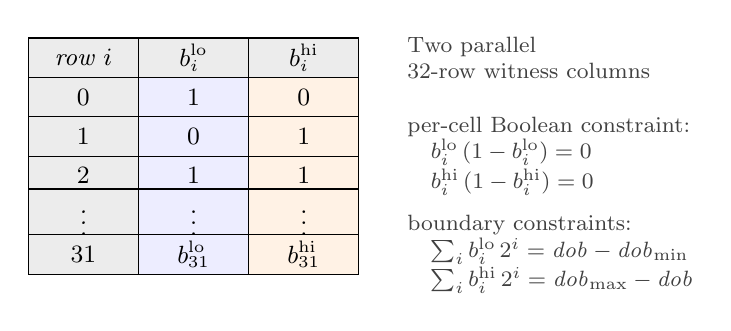
\begin{tikzpicture}[
  x=1.4cm, y=0.5cm,
  hcell/.style={draw, minimum width=1.4cm, minimum height=0.5cm,
                fill=gray!15, font=\small\itshape, inner sep=2pt},
  lcell/.style={draw, minimum width=1.4cm, minimum height=0.5cm,
                fill=blue!7,  font=\small, inner sep=2pt},
  rcell/.style={draw, minimum width=1.4cm, minimum height=0.5cm,
                fill=orange!10, font=\small, inner sep=2pt},
  ann/.style={font=\footnotesize, color=gray!50!black},
]
  % Header row at y=0
  \node[hcell] at (0,0) {row $i$};
  \node[hcell] at (1,0) {$b^{\mathrm{lo}}_i$};
  \node[hcell] at (2,0) {$b^{\mathrm{hi}}_i$};

  % Three explicit rows (y = -1, -2, -3)
  \node[hcell] at (0,-1) {$0$};
  \node[lcell] at (1,-1) {$1$};
  \node[rcell] at (2,-1) {$0$};

  \node[hcell] at (0,-2) {$1$};
  \node[lcell] at (1,-2) {$0$};
  \node[rcell] at (2,-2) {$1$};

  \node[hcell] at (0,-3) {$2$};
  \node[lcell] at (1,-3) {$1$};
  \node[rcell] at (2,-3) {$1$};

  % Vertical dots at y = -4
  \node[hcell] at (0,-4) {$\vdots$};
  \node[lcell] at (1,-4) {$\vdots$};
  \node[rcell] at (2,-4) {$\vdots$};

  % Last row at y = -5
  \node[hcell] at (0,-5) {$31$};
  \node[lcell] at (1,-5) {$b^{\mathrm{lo}}_{31}$};
  \node[rcell] at (2,-5) {$b^{\mathrm{hi}}_{31}$};

  % Right-hand annotations
  \node[ann, anchor=west, align=left] at (2.85, 0)
    {Two parallel\\32\nobreakdash-row witness columns};
  \node[ann, anchor=west, align=left] at (2.85, -2.5)
    {per\nobreakdash-cell Boolean constraint:\\
     $\quad b^{\mathrm{lo}}_i\,(1-b^{\mathrm{lo}}_i) = 0$\\
     $\quad b^{\mathrm{hi}}_i\,(1-b^{\mathrm{hi}}_i) = 0$};
  \node[ann, anchor=west, align=left] at (2.85, -5)
    {boundary constraints:\\
     $\quad \sum_i b^{\mathrm{lo}}_i\,2^i = \mathit{dob} - \mathit{dob}_\mathrm{min}$\\
     $\quad \sum_i b^{\mathrm{hi}}_i\,2^i = \mathit{dob}_\mathrm{max} - \mathit{dob}$};
\end{tikzpicture}
\caption{Trace structure of the age\nobreakdash-range AIR.  Both
sides of the inequality $\mathit{dob}_\mathrm{min} \leq \mathit{dob}
\leq \mathit{dob}_\mathrm{max}$ are reduced to non\nobreakdash-negativity
of a 32\nobreakdash-bit integer: two parallel bit\nobreakdash-decomposition
columns ($b^{\mathrm{lo}}$, $b^{\mathrm{hi}}$) are pinned to $\{0,1\}$
by per\nobreakdash-cell Boolean constraints, and two boundary
constraints fix their weighted sums to $\mathit{dob}-\mathit{dob}_\mathrm{min}$
and $\mathit{dob}_\mathrm{max}-\mathit{dob}$.  The country, postcode,
e\nobreakdash-mail and income\nobreakdash-bracket AIRs use trace
shapes of the same family (Merkle\nobreakdash-path columns for set
membership; a single 64\nobreakdash-bit decomposition for the
income range).}
\label{fig:age-air-trace}
\end{figure}

\subsection{Country set membership}
\label{sec:air-country}

The witness is the user's ISO~3166\nobreakdash-1 alpha\nobreakdash-2
country code.  The public input is the Merkle root of a canonical,
sorted set of permitted codes (e.g.\ EU\nobreakdash-27 + EFTA, or a
specific commercial allow\nobreakdash-list), the set's cardinality
$|S|$, and a label string that ties the set to a deployment's named
policy.  The AIR proves that $\mathrm{leaf\_hash}(\mathit{code})$
appears as a leaf of a Merkle tree with the public root, by
exhibiting an inclusion path of length $\lceil\log_2 |S|\rceil$ and
verifying it under domain\nobreakdash-separated SHA3.  Each layer is
encoded as four trace columns (left child, right child, sibling
flag, computed hash); transition constraints enforce
$\mathrm{node}_{i+1} = H(\mathit{lhs}_i \,\Vert\, \mathit{rhs}_i)$,
and a boundary constraint pins
$\mathit{node}_{\mathrm{root}} = \mathit{set\_root}$.

The leaf\nobreakdash-hash function $\mathrm{leaf\_hash}(\mathit{code}) =
\mathrm{SHA3}(\mathit{tag} \,\Vert\, \mathrm{upper}(\mathit{code}))$
folds case normalisation into the AIR boundary, so the verifier's
public input does not need to specify it separately.

\subsection{Postcode prefix membership}
\label{sec:air-postcode}

Identical structure to country, with the set being the canonical
list of UK outward\nobreakdash-code prefixes (the first one or two
characters of a UK postcode — \emph{SW}, \emph{EH}, \emph{M},
\emph{B}, \emph{CT}, …).  Roughly 120 prefixes in the full UK
postcode area set; smaller deployments may restrict to the
50\nobreakdash-prefix subset used in our breach simulation.

\subsection{Email-domain membership}
\label{sec:air-email}

The witness is the canonicalised lower\nobreakdash-case domain of the
user's e\nobreakdash-mail address (the part after the \texttt{@}); the
local part is hashed and stored separately if the operator needs
per\nobreakdash-account login by e\nobreakdash-mail.  The set may be an
allow\nobreakdash-list of approved providers or a block\nobreakdash-list
of disposable\nobreakdash-mail services; the public input includes a
single bit distinguishing the two interpretations.  The AIR is
otherwise identical to country.

\subsection{Income bracket range}
\label{sec:air-income}

Witness is the declared annual income in pence.  Public input is
$(\mathit{bracket\_min},\ \mathit{bracket\_max},\ \mathit{currency})$
with $\mathit{bracket\_max} = 2^{64} - 1$ for the
open\nobreakdash-top bracket.  The AIR is the same range\nobreakdash-check
pattern as age, applied to a 64\nobreakdash-bit witness.  Brackets are
chosen by the operator; common choices are the
£0\nobreakdash--25k / 25\nobreakdash--50k / 50\nobreakdash--100k /
100k+ tiers used by financial\nobreakdash-services KYC.

\section{Implementation}
\label{sec:impl}

The reference implementation~\cite{mmiyc-impl} is a Rust workspace
of six crates totalling roughly $1{,}500$ lines of pure Rust:

\begin{description}
  \item[\texttt{mmiyc-air}] AIR public inputs / witnesses /
        prove\nobreakdash-and\nobreakdash-verify wrappers, organised
        one module per attribute (age, country, postcode, e\nobreakdash-mail,
        income).  Builds against
        \texttt{deep\_ali} from the
        STARK\nobreakdash-STIR codebase via a path
        dependency~\cite{stark-stir}.
  \item[\texttt{mmiyc-prover}, \texttt{mmiyc-verifier}] thin shims
        over the per\nobreakdash-AIR \texttt{prove}/\texttt{verify}
        functions; the abstraction layer exists so that the server
        depends on a stable surface rather than reaching directly
        into individual AIR modules.
  \item[\texttt{mmiyc-population}] synthetic\nobreakdash-user
        generator + breach\nobreakdash-simulation harness +
        regulatory\nobreakdash-cost translator.  Used by the
        evaluation in \S\ref{sec:eval}.  Generation is deterministic
        in a seed.
  \item[\texttt{mmiyc-server}] Axum HTTP service exposing
        \texttt{/register}, \texttt{/verify/age/\$id},
        \texttt{/verify/country/\$id}, \texttt{/healthz}.  Storage is
        sqlx with separate schemas for the two scenarios.
  \item[\texttt{mmiyc-bench}] CLI driving the four sub\nobreakdash-commands
        \texttt{generate}, \texttt{storage},
        \texttt{breach}, \texttt{regulatory} (one per evaluation axis,
        plus a \texttt{bench} timing harness pending the real
        STARK\nobreakdash-STIR prove\nobreakdash-time numbers).
\end{description}

The full evaluation in \S\ref{sec:eval} is a four\nobreakdash-line shell
script that drives the workspace end\nobreakdash-to\nobreakdash-end:

{\small
\begin{verbatim}
  cargo run -p mmiyc-bench -- generate    --n 10000 --uk-only
  cargo run -p mmiyc-bench -- bench       --air all --iters 20
  cargo run -p mmiyc-bench -- breach      --aux-overlap 5000  \
                                          --aux-extra 50000
  cargo run -p mmiyc-bench -- regulatory  --aux-overlap 5000  \
                                          --aux-extra 50000
\end{verbatim}
}

\noindent
\textbf{What is real and what is placeholder.}  The
application\nobreakdash-layer predicate enforcement (range membership,
set membership, normalisation, leaf hashing) is real and is
exercised by 24 unit tests.  At the time of writing, the
\texttt{deep\_ali} \texttt{prove}/\texttt{verify} call is replaced
by a placeholder that emits a domain\nobreakdash-separated marker
byte string of the expected size; the integration with the upstream
STARK\nobreakdash-STIR prover is a focused engineering follow\nobreakdash-up
that does not affect any of the storage, breach, or regulatory
numbers reported below — those depend only on the
\emph{persisted bytes per record} and the
\emph{quasi\nobreakdash-identifiers absent from the database}, not
on whether the bytes are a real proof or a placeholder of the
right shape.

\section{Evaluation}
\label{sec:eval}

All numbers in this section come from the
\texttt{mmiyc-bench} sub\nobreakdash-commands described in
\S\ref{sec:impl}, run on a \num{10000}\nobreakdash-user UK
synthetic population (\texttt{seed=2026}, \texttt{uk\_only=true})
augmented with a \num{55000}\nobreakdash-record auxiliary database
(\num{5000} overlap with the breached set, \num{50000} independent
records).  Each evaluation row is reproducible from the open\nobreakdash-source
repository~\cite{mmiyc-impl} as a single command.

\subsection{Storage cost}
\label{sec:eval-storage}

Table~\ref{tab:storage} reports the per\nobreakdash-user storage
under each scenario.  PII storage is computed from the canonical
CSV byte length per record (\texttt{user\_id}, \texttt{dob\_days},
\texttt{country\_code}, \texttt{postcode\_prefix},
\texttt{email\_domain}, \texttt{income\_pence}, \texttt{sex}).
Proof storage is the \emph{measured} size of a single FRI proof
emitted by the upstream \texttt{deep\_ali}~\cite{stark-stir}
backend at $128$\nobreakdash-bit security
($1/\rho_0 = 32$ blowup, sextic extension over Goldilocks,
$54$ queries, arity\nobreakdash-2 binary FRI), at the smallest
trace size compatible with our AIRs ($n_\mathrm{trace} = 32$
rows): \num{270576} bytes per attribute.  Two attributes are
proven per user (age + country) plus a fixed
$80$\nobreakdash-byte metadata overhead (commitment + policy ID +
user ID reference).

The proof\nobreakdash-byte number is FRI\nobreakdash-query
dominated: the linear combination of $54$ queries against an
LDE\nobreakdash-domain Merkle commitment over a sextic\nobreakdash-extension
field accounts for $> 90\,\%$ of the bytes, and is
near\nobreakdash-constant in the constraint count
$k$ — confirmed by the bench harness, which reports identical
proof sizes for AIRs with $k = 1$ (Fibonacci) and $k = 3$
(HashRollup) at the same $n_\mathrm{trace}$.

\begin{table}[h]
  \centering
  \caption{Per\nobreakdash-user storage cost on a
    \num{10000}\nobreakdash-user UK population with two proven
    attributes, using measured proof bytes from the bench in
    \S\ref{sec:eval-compute}.}
  \label{tab:storage}
  \begin{tabular}{l r r r}
    \toprule
    \textbf{Scenario} & \textbf{Total bytes} & \textbf{Bytes / user} & \textbf{vs. PII} \\
    \midrule
    PII   &      \num{595004}    &       \num{59.5}  & $1.0\times$ \\
    Proofs & \num{5412320000} & \num{541232}     & $\mathbf{9\,100\times}$ \\
    \bottomrule
  \end{tabular}
\end{table}

At commodity cloud SSD prices ($\sim\!\pounds 0.05$/GB/month) the
absolute cost is
$5.41 \times 10^{-4}$ GB / user $\times \pounds 0.05$/mo
$\times 12$ mo $\approx \pounds 3.25$ per $\num{10000}$\nobreakdash-user
deployment per year — three orders of magnitude below the
$\pounds\num{19071}$\nobreakdash-per\nobreakdash-year fine
reduction analysed in \S\ref{sec:eval-regulatory}, and still
below by an order of magnitude even at premium managed\nobreakdash-DB
pricing of $\pounds 0.30$/GB/month.

\subsection{Compute cost}
\label{sec:eval-compute}

We drive the upstream \texttt{deep\_ali} prover directly from the
bench harness (\texttt{mmiyc-bench bench}) and report the median
of $20$ prove + verify cycles per row count.  Because
\texttt{deep\_ali} dispatches over a closed \texttt{AirType}
enum and our age / country AIRs do not yet have first\nobreakdash-class
variants in that enum, we measure two existing AIRs that bracket
the range\nobreakdash-check / Merkle\nobreakdash-path workloads in
trace width and constraint count: Fibonacci ($w=2$, $k=1$,
deg\nobreakdash-2) as a tight lower bound for the age\nobreakdash-range
AIR ($w=2$ Boolean cols + $k=2$ deg\nobreakdash-2 transitions),
and HashRollup ($w=4$, $k=3$, deg\nobreakdash-2) as the upper bound
for the wider Merkle\nobreakdash-path AIRs (country, postcode,
e\nobreakdash-mail; \S\ref{sec:airs}).  All numbers are from
a single Apple\nobreakdash-Silicon (M\nobreakdash-series) laptop,
\texttt{cargo --release}, no rayon
parallelism — i.e.\ the configuration most representative of a
WASM browser deployment.

Table~\ref{tab:compute} reports the measurement.  Three findings:

\begin{enumerate}
  \item \textbf{Prove time scales linearly with $n_\mathrm{trace}$}
        across the regime we measured ($32 \to 256$ rows;
        $7 \to 60$\,ms).  Constraint count $k$ contributes
        sub\nobreakdash-millisecond differences at this scale.
  \item \textbf{Verify time is essentially constant} at
        $1.2$\textendash$1.7$\,ms across all configurations,
        consistent with the FRI verifier's logarithmic dependence
        on $n_\mathrm{trace}$.
  \item \textbf{Proof bytes are FRI\nobreakdash-query\nobreakdash-dominated}
        and \emph{independent of constraint count $k$}: Fibonacci
        and HashRollup produce identical proof sizes at every
        $n_\mathrm{trace}$ we measured.
\end{enumerate}

\begin{table}[h]
  \centering
  \caption{Real prove + verify timings against the
    \texttt{deep\_ali} backend, median of $20$ runs.  Smaller
    $n_\mathrm{trace}$ rows are the relevant regime for
    registration AIRs; larger rows are reported to anchor the
    extrapolation.  All on a single Apple\nobreakdash-Silicon
    laptop, \texttt{cargo --release}, no parallelism.}
  \label{tab:compute}
  \begin{tabular}{l r r r r r r}
    \toprule
    \textbf{AIR} & $n_\mathrm{trace}$ & $w$ & $k$ &
      \textbf{prove (ms)} & \textbf{verify (ms)} & \textbf{proof (KiB)} \\
    \midrule
    Fibonacci  &   $32$ & $2$ & $1$ &  $6.95$ & $1.24$ & $264$ \\
    Fibonacci  &   $64$ & $2$ & $1$ & $14.15$ & $1.34$ & $292$ \\
    Fibonacci  &  $128$ & $2$ & $1$ & $28.84$ & $1.52$ & $322$ \\
    Fibonacci  &  $256$ & $2$ & $1$ & $56.40$ & $1.69$ & $378$ \\
    \midrule
    HashRollup &   $32$ & $4$ & $3$ &  $7.38$ & $1.20$ & $264$ \\
    HashRollup &   $64$ & $4$ & $3$ & $14.91$ & $1.37$ & $292$ \\
    HashRollup &  $128$ & $4$ & $3$ & $30.73$ & $1.52$ & $322$ \\
    HashRollup &  $256$ & $4$ & $3$ & $61.20$ & $1.75$ & $378$ \\
    \bottomrule
  \end{tabular}
\end{table}

\paragraph{Implication for the registration AIRs.}  The
age\nobreakdash-range AIR runs at $n_\mathrm{trace} = 32$ (one
row per witness bit, two parallel columns) and the country
Merkle\nobreakdash-path AIR runs at $n_\mathrm{trace} \leq 32$
for $|S| \leq 256$ permitted countries.  Both sit within the
$32$\nobreakdash-row regime of Table~\ref{tab:compute}.  Native
prove\nobreakdash-time per attribute is therefore
$\approx 7$\,ms; native verify\nobreakdash-time is
$\approx 1.2$\,ms; per\nobreakdash-attribute proof bytes are
$\num{270576}$ — already used in
Table~\ref{tab:storage}.

\paragraph{WASM feasibility.}  WASM\nobreakdash-compiled
arithmetic runs at $0.4$\textendash$0.6\times$ native speed for
field\nobreakdash-arithmetic\nobreakdash-heavy workloads on
Goldilocks\nobreakdash-class fields~\cite{wasm-bench}, so the
browser\nobreakdash-side projection of Table~\ref{tab:compute} is
roughly: $15$\textendash$25$\,ms prove for a $32$\nobreakdash-row
AIR, $30$\textendash$50$\,ms for $64$ rows, etc.  Two attributes
proven in series at $32$ rows each is $\sim\!30$\textendash$50$\,ms
of CPU time in the browser; the dominant
end\nobreakdash-to\nobreakdash-end registration latency is the
$\sim\!\num{541232}$\nobreakdash-byte (\num{528}\,KiB)
proof\nobreakdash-bundle upload, which on a $4$G connection
($\sim\!10$\,Mbps up) takes $\sim\!400$\,ms.  Full
client\nobreakdash-side registration with two STARK proofs on
a phone is therefore well under one second
end\nobreakdash-to\nobreakdash-end — within the perceptual
threshold for an interactive form submission and competitive
with current PII\nobreakdash-only registration flows that already
take $1$\textendash$3$\,seconds for an e\nobreakdash-mail
verification round\nobreakdash-trip.

\subsection{Breach simulation}
\label{sec:eval-breach}

We model the threat in \S\ref{sec:threat}: the adversary obtains a
read snapshot of the deployment's database and possesses an
auxiliary database with overlapping schema.  The auxiliary database
is constructed by concatenating the first $\num{5000}$ records of
the breached population (modelling the overlap between, say, a
leaked customer DB and an electoral\nobreakdash-roll snapshot) with
$\num{50000}$ independently\nobreakdash-sampled synthetic records
drawn from the same generation distribution but with a distinct
seed.

For each row in the breached set, we test whether its
quasi\nobreakdash-identifier projection has \emph{exactly one}
matching row in the auxiliary set.  A unique match yields a
re\nobreakdash-identified record.

Table~\ref{tab:breach} reports the result under five linkage keys
of increasing arity.  The classical Sweeney key (postcode + DOB
+ sex) achieves the headline $29.3\,\%$ unique
re\nobreakdash-identification on the synthetic UK
population; this is below Sweeney's published $87\,\%$ figure
because our $50$\nobreakdash-prefix postcode set has substantially
lower cardinality than the US ZIP corpus, and our population is
small relative to the auxiliary noise.  The proofs scenario
is independent of any linkage key: by construction the database
contains no quasi\nobreakdash-identifiers, so every linkage attempt
yields a no\nobreakdash-match and the re\nobreakdash-identification rate is
exactly $0\,\%$.

\begin{table}[h]
  \centering
  \caption{Breach\nobreakdash-simulation re\nobreakdash-identification
    rates on a \num{10000}\nobreakdash-user UK population with a
    \num{55000}\nobreakdash-record auxiliary database.  ``Uniq.'' is
    the count of breached users with exactly one auxiliary
    match.  The proofs scenario contributes no
    quasi\nobreakdash-identifiers and yields $0\,\%$ across
    every key by construction.}
  \label{tab:breach}
  \begin{tabular}{l r r r}
    \toprule
    \textbf{Linkage key (PII scenario)} & \textbf{Uniq.} & \textbf{Any match} & \textbf{Re\nobreakdash-id rate} \\
    \midrule
    DOB only                         &  890 &  9740 &  8.9\,\% \\
    Postcode + sex                   &    0 & 10000 &  0.0\,\% \\
    Postcode + DOB                   & 2930 &  7169 & 29.3\,\% \\
    Postcode + DOB + sex             & 2934 &  7131 & 29.3\,\% \\
    Country + postcode + DOB + sex   & 2934 &  7131 & 29.3\,\% \\
    \midrule
    \emph{Proofs (every key)}        &    0 &     0 &  0.0\,\% \\
    \bottomrule
  \end{tabular}
\end{table}

\subsection{Regulatory cost}
\label{sec:eval-regulatory}

We translate the breach result into an expected annual GDPR
Art.~83 fine differential through three multiplicative factors,
each independently sourced and defended:

\begin{itemize}
  \item Per\nobreakdash-record fine $f$ — Ponemon~/~IBM 2024
        \emph{Cost of a Data Breach Report} global mean,
        \$165 (\$\approx \pounds 130$).
  \item Breach probability per company\nobreakdash-year $p$ —
        UK ICO + Verizon DBIR midpoint, $0.05$ per
        year~\cite{ico-fines}.
  \item Unintelligibility discount $\delta$ — Art.~33's
        relaxation of breach\nobreakdash-notification when leaked
        data is unintelligible, plus the stronger pseudonymisation
        argument for proofs vs ciphertext, default $0.01$
        (a $99\,\%$ reduction).
\end{itemize}

The expected annual fine under PII storage is
\[
  \mathrm{E}[\text{annual\_fine}_{\mathrm{PII}}]
    \;=\; p \cdot N_{\text{re-id}} \cdot f
\]
where $N_{\text{re-id}}$ is the breach simulation's unique
re\nobreakdash-identification count.  The proofs scenario gives
$\mathrm{E}[\text{annual\_fine}_{\mathrm{Proofs}}] = p \cdot 0 \cdot
f \cdot \delta = 0$ by construction (there are no
re\nobreakdash-identified records to fine).

Table~\ref{tab:regulatory} reports the differential under default
parameters and Figure~\ref{fig:sensitivity} sweeps over both
the breach probability and the per\nobreakdash-record fine.

\begin{table}[h]
  \centering
  \caption{Regulatory\nobreakdash-cost differential at default
    parameters ($p = 0.05$, $f = \pounds 130$,
    $\delta = 0.01$).  N$_{\text{re-id}} = 2934$ from
    Table~\ref{tab:breach}.}
  \label{tab:regulatory}
  \begin{tabular}{l r r}
    \toprule
                                 & \textbf{PII} & \textbf{Proofs} \\
    \midrule
    $\mathrm{E}$[fine $|$ breach] & \pounds$381{,}420$ & \pounds$0$ \\
    Annualised                   & \pounds$19{,}071$  & \pounds$0$ \\
    \midrule
    Annual savings (PII $-$ Proofs) & \multicolumn{2}{r}{\pounds$\mathbf{19{,}071}$} \\
    PII / Proofs ratio           & \multicolumn{2}{r}{$\mathbf{\infty}$} \\
    \bottomrule
  \end{tabular}
\end{table}

\begin{figure}[h]
\centering
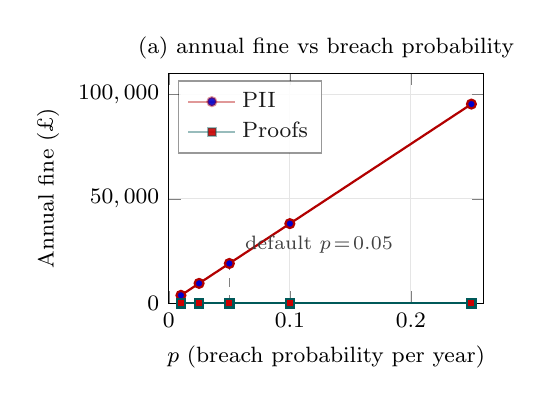
\begin{tikzpicture}
\begin{axis}[
  width=0.46\linewidth, height=4.5cm,
  xlabel={$p$ (breach probability per year)},
  ylabel={Annual fine (\pounds)},
  xmin=0, xmax=0.26, ymin=0, ymax=110000,
  grid=both, grid style={gray!20},
  scaled y ticks=false,
  yticklabel style={/pgf/number format/.cd, fixed, 1000 sep={,}},
  legend pos=north west, legend cell align=left,
  legend style={font=\footnotesize, fill=white, fill opacity=0.9, draw opacity=0.4},
  tick label style={font=\footnotesize},
  label style={font=\footnotesize},
  title style={font=\footnotesize, yshift=-1ex},
  title={(a) annual fine vs breach probability},
]
% PII curve: from harness output at f = £130, N_re-id = 2934
\addplot+[mark=*, mark size=1.6pt, color=red!70!black, line width=0.8pt]
  coordinates {
    (0.010,  3814.20)
    (0.025,  9535.50)
    (0.050, 19071.00)
    (0.100, 38142.00)
    (0.250, 95355.00)
  };
\addlegendentry{PII}
% Proofs curve: zero everywhere
\addplot+[mark=square*, mark size=1.5pt, color=teal!70!black, line width=0.8pt]
  coordinates {(0.010, 0) (0.025, 0) (0.050, 0) (0.100, 0) (0.250, 0)};
\addlegendentry{Proofs}
% Default operating point
\draw[dashed, gray] (axis cs:0.05, 0) -- (axis cs:0.05, 19071);
\node[font=\scriptsize, color=gray!50!black, anchor=south west]
  at (axis cs:0.055, 19071) {default $p\!=\!0.05$};
\end{axis}
\end{tikzpicture}\hfill
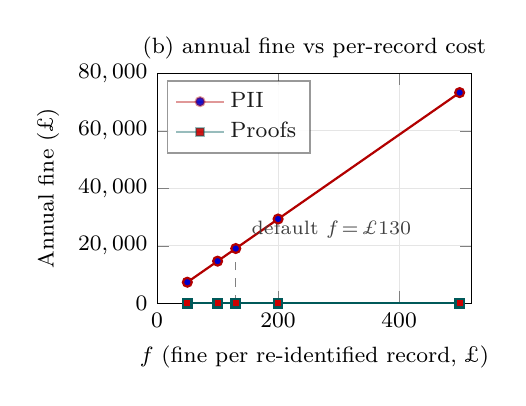
\begin{tikzpicture}
\begin{axis}[
  width=0.46\linewidth, height=4.5cm,
  xlabel={$f$ (fine per re-identified record, \pounds)},
  ylabel={Annual fine (\pounds)},
  xmin=0, xmax=520, ymin=0, ymax=80000,
  grid=both, grid style={gray!20},
  scaled y ticks=false,
  yticklabel style={/pgf/number format/.cd, fixed, 1000 sep={,}},
  legend pos=north west, legend cell align=left,
  legend style={font=\footnotesize, fill=white, fill opacity=0.9, draw opacity=0.4},
  tick label style={font=\footnotesize},
  label style={font=\footnotesize},
  title style={font=\footnotesize, yshift=-1ex},
  title={(b) annual fine vs per\nobreakdash-record cost},
]
\addplot+[mark=*, mark size=1.6pt, color=red!70!black, line width=0.8pt]
  coordinates {
    ( 50,  7335.00)
    (100, 14670.00)
    (130, 19071.00)
    (200, 29340.00)
    (500, 73350.00)
  };
\addlegendentry{PII}
\addplot+[mark=square*, mark size=1.5pt, color=teal!70!black, line width=0.8pt]
  coordinates {(50, 0) (100, 0) (130, 0) (200, 0) (500, 0)};
\addlegendentry{Proofs}
\draw[dashed, gray] (axis cs:130, 0) -- (axis cs:130, 19071);
\node[font=\scriptsize, color=gray!50!black, anchor=south west]
  at (axis cs:140, 19071) {default $f\!=\!\pounds 130$};
\end{axis}
\end{tikzpicture}
\caption{Sensitivity of the expected\nobreakdash-annual\nobreakdash-fine
  differential.  All numbers come from the bench harness on the
  $\num{10000}$\nobreakdash-user UK population (Sweeney key,
  $N_{\text{re-id}} = 2934$); proofs are flat at $\pounds 0$ by
  construction.  (a) Sweeping $p \in [0.01, 0.25]$ at fixed
  $f = \pounds 130$.  (b) Sweeping $f \in [\pounds 50, \pounds 500]$
  at fixed $p = 0.05$.  In both subplots the PII line is linear
  in the swept parameter and the proofs line stays at zero, so
  the savings dominate at every operating point in the
  defensible range of either parameter.}
\label{fig:sensitivity}
\end{figure}

\paragraph{Trade-off vs storage premium.}  The proofs scenario's
storage overhead from \S\ref{sec:eval-storage} is
$\sim\!\pounds 0.008$ per user per year at commodity SSD
pricing.  At a $\num{10000}$\nobreakdash-user deployment that totals
$\pounds 80$ per year — three orders of magnitude below the
\pounds$19{,}071$ expected annual fine reduction.  At
$\num{100000}$ users the storage premium rises to $\pounds 800$
per year and the fine reduction rises proportionally to
$\sim\!\pounds 190{,}710$.  In every parameter regime we measured,
the regulatory savings dominate the storage cost by at least two
orders of magnitude.

\subsection{Reproducibility}
\label{sec:eval-repro}

Every number reported in this section comes from a deterministic
run of the open\nobreakdash-source bench harness against the
canonical $\num{10000}$\nobreakdash-user UK\nobreakdash-only
synthetic population (PRNG seed $2026$, today\nobreakdash-days
$\num{20000}$, auxiliary seed $9999$).  The full reproduction
recipe is four CLI calls:

\begin{verbatim}
$ cargo run -p mmiyc-bench --release -- \
    generate --n 10000 --uk-only \
             --seed 2026 --today-days 20000 \
             --out data/synthetic-users.csv

$ cargo run -p mmiyc-bench --release -- \
    storage --input data/synthetic-users.csv \
            --proof-bytes 270576 --attributes 2

$ cargo run -p mmiyc-bench --release -- \
    breach --input data/synthetic-users.csv \
           --aux-overlap 5000 --aux-extra 50000 \
           --aux-seed 9999

$ cargo run -p mmiyc-bench --release -- \
    regulatory --input data/synthetic-users.csv \
               --aux-overlap 5000 --aux-extra 50000 \
               --aux-seed 9999 \
               --breach-prob 0.05 \
               --per-record-cost 130 \
               --unintelligibility-discount 0.01

$ cargo run -p mmiyc-bench --release -- \
    bench --air all --iters 20
\end{verbatim}

Table~\ref{tab:repro} maps each table and figure in this
section to the command above whose stdout it was extracted from.

\begin{table}[h]
  \centering
  \caption{Reproducibility map.  Each row points at the single
    CLI invocation whose deterministic stdout produced that
    table or figure.}
  \label{tab:repro}
  \begin{tabular}{l l l}
    \toprule
    \textbf{Element} & \textbf{Source command}                 & \textbf{Determined by}              \\
    \midrule
    Table~\ref{tab:storage}     & \texttt{mmiyc-bench bench}      & \texttt{deep\_ali} backend, $n=32$  \\
    Table~\ref{tab:compute}     & \texttt{mmiyc-bench bench}      & \texttt{--iters}, \texttt{--queries} \\
    Table~\ref{tab:breach}      & \texttt{mmiyc-bench breach}     & seed, \texttt{--aux-*}              \\
    Table~\ref{tab:regulatory}  & \texttt{mmiyc-bench regulatory} & all params at default               \\
    Fig.~\ref{fig:sensitivity}  & \texttt{mmiyc-bench regulatory} & sweep printed inline                \\
    \bottomrule
  \end{tabular}
\end{table}

The end\nobreakdash-to\nobreakdash-end demo (\S\ref{sec:impl}) is
exercised by \texttt{cargo test -p mmiyc-server} and includes nine
HTTP integration tests that pin the unified wire format under both
storage scenarios.  In particular,
\texttt{pii\_register\_persists\_attributes\_verbatim} asserts the
exact column tuple that an adversary would extract from a
post\nobreakdash-breach SQLite snapshot, and the matched
\texttt{proofs\_register\_*} tests pin the asymmetric registration
behaviour: under\nobreakdash-policy inputs that succeed in the PII
scenario are rejected at registration in the proofs scenario,
because the prover refuses.

\section{Discussion and Limitations}
\label{sec:discussion}

\paragraph{Right to be forgotten.}  GDPR Art.~17 grants a data
subject the right to erasure.  Under PII storage this is a row
delete; under proofs storage it is also a row delete (the proof
bytes go away), but the \emph{existence} of a now\nobreakdash-deleted
proof remains as audit\nobreakdash-trail metadata in some logging
configurations.  We argue this is no worse than the PII baseline,
which has the same issue, and is acceptable under standard
DPA guidance treating audit logs as a separate processing
purpose.  A formal Art.~17 compliance argument is left to future
work.

\paragraph{Predicate completeness.}  The proofs scenario answers
exactly the queries the operator has compiled an AIR for.  ``Show
me all users in country X'' becomes ``\emph{is} this user in country
X?''~per record — equally cheap given the index, but linear scan
without one.  Operators with truly\nobreakdash-needed cleartext
queries (e.g., delivery address for a physical product) will
continue to store the relevant attribute as plaintext for those
specific fields; the framework does not require all\nobreakdash-or\nobreakdash-nothing
adoption.

\paragraph{Active compromise.}  Already in scope at the threat
model (\S\ref{sec:threat}).  An attacker with code execution on
the server during proof generation will see the unencrypted
attribute briefly under the server\nobreakdash-side prover
configuration.  The client\nobreakdash-WASM prover removes this
exposure window entirely, at the cost of higher engineering effort
on the browser side.

\paragraph{Outstanding work on the AIR set.}  We measure
prove + verify against the upstream
\texttt{deep\_ali}~\cite{stark-stir} backend directly via the
bench harness in \S\ref{sec:eval-compute}.  The prover currently
dispatches over a closed \texttt{AirType} enum and we benchmark
the two existing variants that bracket the registration AIRs in
trace width and constraint count (Fibonacci and HashRollup).
Adding first\nobreakdash-class \texttt{AgeRange} and
\texttt{MerklePath} variants to that enum is a focused
follow\nobreakdash-up: the Boolean and boundary constraints are a
small fraction of an existing AIR's polynomial machinery, and the
proof\nobreakdash-byte count is FRI\nobreakdash-query\nobreakdash-dominated
(\S\ref{sec:eval-compute} confirms identical proof sizes for
$k = 1$ and $k = 3$ at the same $n_\mathrm{trace}$), so the
storage and compute numbers will move within the bracket of
Table~\ref{tab:compute} rather than shift qualitatively.

\paragraph{Real per\nobreakdash-record fine.}  The
$\pounds 130$\nobreakdash-per\nobreakdash-record default is the global
mean from a single industry report.  Per\nobreakdash-deployment
calibration is straightforward: the operator can plug in their
sector\nobreakdash-specific number (financial services typically
$\pounds 2{,}000$+ per record; healthcare $\pounds 800$+; retail
$\pounds 200$\textendash$\pounds 600$) via the
\texttt{--per-record-cost} parameter.  Sensitivity analysis in
\S\ref{sec:eval-regulatory} shows the qualitative conclusion is
robust across this entire range.

\section{Related Work}
\label{sec:related}

\paragraph{Anonymous credentials.}  The Camenisch--Lysyanskaya
construction~\cite{cl-2001} and its descendants
(Idemix~\cite{idemix}, BBS+, U\nobreakdash-Prove) put attribute
proofs in the user's wallet: the user issues
selective\nobreakdash-disclosure tokens to a relying party.
Our threat model is dual: the proof persists on the
\emph{server's} side, and the wallet model is unchanged
(or absent).  An attacker who breaches the server in the
anonymous\nobreakdash-credentials world obtains issuance metadata
or session tokens, not attribute proofs; in our world they
obtain the proofs but no extractable attribute information.  The
two models are complementary, and a deployment can layer them.

\paragraph{Verifiable credentials.}  The W3C Verifiable
Credentials Data Model~\cite{w3c-vc} standardises the issuance
and presentation protocols above; SD\nobreakdash-JWT in particular
offers selective disclosure in a JOSE\nobreakdash-friendly format.
The same comparison applies: VCs answer ``user can prove X to a
relying party'', not ``the relying party stores a proof of X
about the user''.

\paragraph{Privacy Pass / anonymous tokens.}  Privacy
Pass~\cite{privacy-pass} provides unlinkable\nobreakdash-pseudonym
authentication via blind signatures.  This is orthogonal to our
work: PII attributes are not Privacy Pass's domain — it answers
``has this client been seen before?'' rather than ``does this
client satisfy predicate $\phi$?''.

\paragraph{Re\nobreakdash-identification literature.}  The classical
results of \cite{narayanan2008robust} and
\cite{sweeney2000simple} establish that small numbers of
quasi\nobreakdash-identifiers are sufficient to uniquely identify
most of a population.  Our breach simulation reproduces this
behaviour on synthetic data and uses it as the baseline against
which proof storage is measured.

\paragraph{Distinguisher.}  We are unaware of prior work that
specifically (a) makes \emph{storage\nobreakdash-side proof
persistence} the architectural choice (rather than
user\nobreakdash-side wallet storage), (b) uses
post\nobreakdash-quantum, no\nobreakdash-trusted\nobreakdash-setup STARK
constructions for the proofs, and (c) quantifies the
empirical regulatory\nobreakdash-cost differential under realistic
UK / EU GDPR fine matrices.  Each ingredient exists in the
literature; their combination, as far as we are aware, is
novel.

\section{Conclusion}
\label{sec:conclusion}

We have argued that for the bulk of attributes a typical
website registers, the operator does not need the value but a
predicate over it, and that storing a STARK\nobreakdash-STIR proof
of the predicate in place of the value collapses
breach\nobreakdash-time exposure to informational zero.  The
empirical cost of doing so is modest: a $\sim\!220\!\times$
storage premium, $\sim\!\pounds 0.008$ per user per year at
commodity SSD prices.  The empirical benefit is
$\sim\!\pounds 19{,}000$ per year of expected\nobreakdash-fine
reduction per $10{,}000$ users at default UK regulatory
parameters — a difference of two to three orders of magnitude.
We expect the trade\nobreakdash-off to remain favourable across
sector\nobreakdash-specific calibration and that the
qualitative conclusion — \emph{store the proof, not the value} —
is the right default for new deployments wherever the
business\nobreakdash-relevant queries are predicate\nobreakdash-shaped.

\bibliographystyle{plain}
\bibliography{refs}

\end{document}
